\documentclass{article}
\usepackage{fancyhdr}
\usepackage{lastpage}
\usepackage{amsmath}
\usepackage{amssymb}
\usepackage{amsthm}
\usepackage{tabstackengine}
\usepackage[margin=1in]{geometry}
\usepackage{graphicx}
\graphicspath{ {./} }
\TABstackMath
\TABbinary

\pagestyle{fancy}
\setlength\headheight{28pt}
\addtolength{\headheight}{\baselineskip}
\fancyhf{}
\renewcommand{\headrulewidth}{0pt}
\lhead{Math 251 - Shuichi Masuda\\Juno Suárez\\\today}
\rfoot{Page \thepage \hspace{1pt} of \pageref{LastPage}}

\renewcommand\thesubsection{\arabic{subsection}.}
\renewcommand\thesubsubsection{\alph{subsubsection})}

\begin{document}

\section*{Graded Problem \# 2}

\subsection{}
\emph{Graph sketched on cover sheet.}

\subsection{}
Given
$$
f(x)=xe^x
$$

\subsubsection{}
Then
\\

\tabbedLongunderstack[l]{
  f'(x) =& x(e^x)' + e^x(x)' \\
  \phantom{f'(x)} =& x(e^x) + e^x(1) \\
  \phantom{f'(x)} =& \boxed{x(e^x) + e^x}
}
\quad
\Longunderstack[l]{
  Product rule \\
  Logarithmic derivative
}

\subsubsection{}
Then
\\

\tabbedLongunderstack[l]{
  f''(x) =& (xe^x + e^x)' \\
  \phantom{f''(x)} =& (xe^x)' + (e^x)' \\
  \phantom{f''(x)} =& (xe^x + e^x) + (e^x) \\
  \phantom{f''(x)} =& \boxed{xe^x + 2e^x}
}
\quad
\Longunderstack[l]{
  $f'$ derived in 2.a\\
  Linearity property of derivative \\
  \\
  Simplify
}

\subsubsection{}
Then
\\

\tabbedLongunderstack[l]{
  f''(x) =& (xe^x)' + (2e^x)' \\
  \phantom{f''(x)} =& (xe^x + e^x) + 2e^x \\
  \phantom{f''(x)} =& \boxed{xe^x + 3e^x}
}
\quad
\Longunderstack[l]{
  $f''$ derived in 2.a, Linearity property of derivative
}


\subsubsection{}
Based on the pattern in 2.a-c, I conjecture that
\\

\tabbedLongunderstack[l]{
  f^{(1000)}(x) =& xe^x + 1000e^x
}
\quad
\Longunderstack[l]{
\phantom{ }
}

\subsubsection{}
More generally, for the $n^{\text{th}}$ derivative of $f$, I conjecture:
\\

\tabbedLongunderstack[l]{
  f^{(n)}(x) =& xe^x + ne^x
}
\quad
\Longunderstack[l]{
\phantom{ }
}

\subsection{}
For the function
$$
f(x) = \frac{3x+5}{1+x}
$$

\subsubsection{}
The equation for the tangent line to $f(x)$ at $x=1$ is given by the point-slope equation
$$
y = m(x-x_0) + y_0
$$
where the point $(x_0, y_0)$ is given by $(x, f(x))$ and $m$ is given by $f'(x)$. We're given $x_0=1$, so we must solve for $y_0 = f(1)$ and $m = f'(1)$.
\\

\tabbedLongunderstack[l]{
  f(1) =& \frac{3(1) + 5}{1+1}\\
  \phantom{f(1)} =& \frac{8}{2}\\
  &\\
  \phantom{f(1)} =& \boxed{4}
}
\\
\\
\\
so for the point $(1, 4)$ we have $y = m(x-1) + 4$ and must next find $m$. First we compute $f'(x)$:
\\

\tabbedLongunderstack[l]{
  f'(x) =& \frac{(1+x)(3x+5)' - (3x+5)(1+x)'}{(1+x)^2} \\
  & \\
  \phantom{f'(x)} =& \frac{(1+x)(3) - (3x+5)(1)}{(1+x)^2} \\
  & \\
  \phantom{f'(x)} =& \frac{3+3x - 3x - 5}{(1+x)^2} \\
  & \\
  \phantom{f'(x)} =& \boxed{\frac{-2}{(1+x)^2}}
}
\quad
\Longunderstack[l]{
  Quotient rule\\
  \\
  Power rule\\
}
\\
\\
\\
And finally we compute $m$ by $m=f'(1)$:
\\

\tabbedLongunderstack[l]{
  f'(1) =& \frac{-2}{(1+1)^2} \\
  & \\
  \phantom{f'(1)} =& \frac{-2}{(2)^2} \\
  & \\
  \phantom{f'(1)} =& \frac{-2}{4} \\
  & \\
  \phantom{f'(1)} =& \boxed{-\frac{1}{2}}
}
\quad
\Longunderstack[l]{
  \phantom{ }
}
\\
\\

Giving us our complete equation:
$$
\boxed{y = -\frac{1}{2}(x-1)+4}
$$

\subsubsection{}
To find the equation for a line perpendicular to another line, recall that the slope of the perpendicular line is the negative reciprocal. In the case of the line in 3.a, the slope is $-\frac{1}{2}$. The reciprocal of $-\frac{1}{2}$ is $-2$, and the negation is $2$. Since the equation in
3.a is already in point-slope form, if we plug this new slope into the same form it will give us the equation for a perpendicular line passing through the same point:
$$
\boxed{y=2(x-1)+4}
$$

\subsubsection{}
Graphed in GeoGebra, the equation derived in 3.a appears to be tangent
to $f(x)$ at $x=1$ and the equation derived in 3.b appears to be perpendicular
to the tangent of $f(x)$ at $x=1$. \emph{See graph below.}

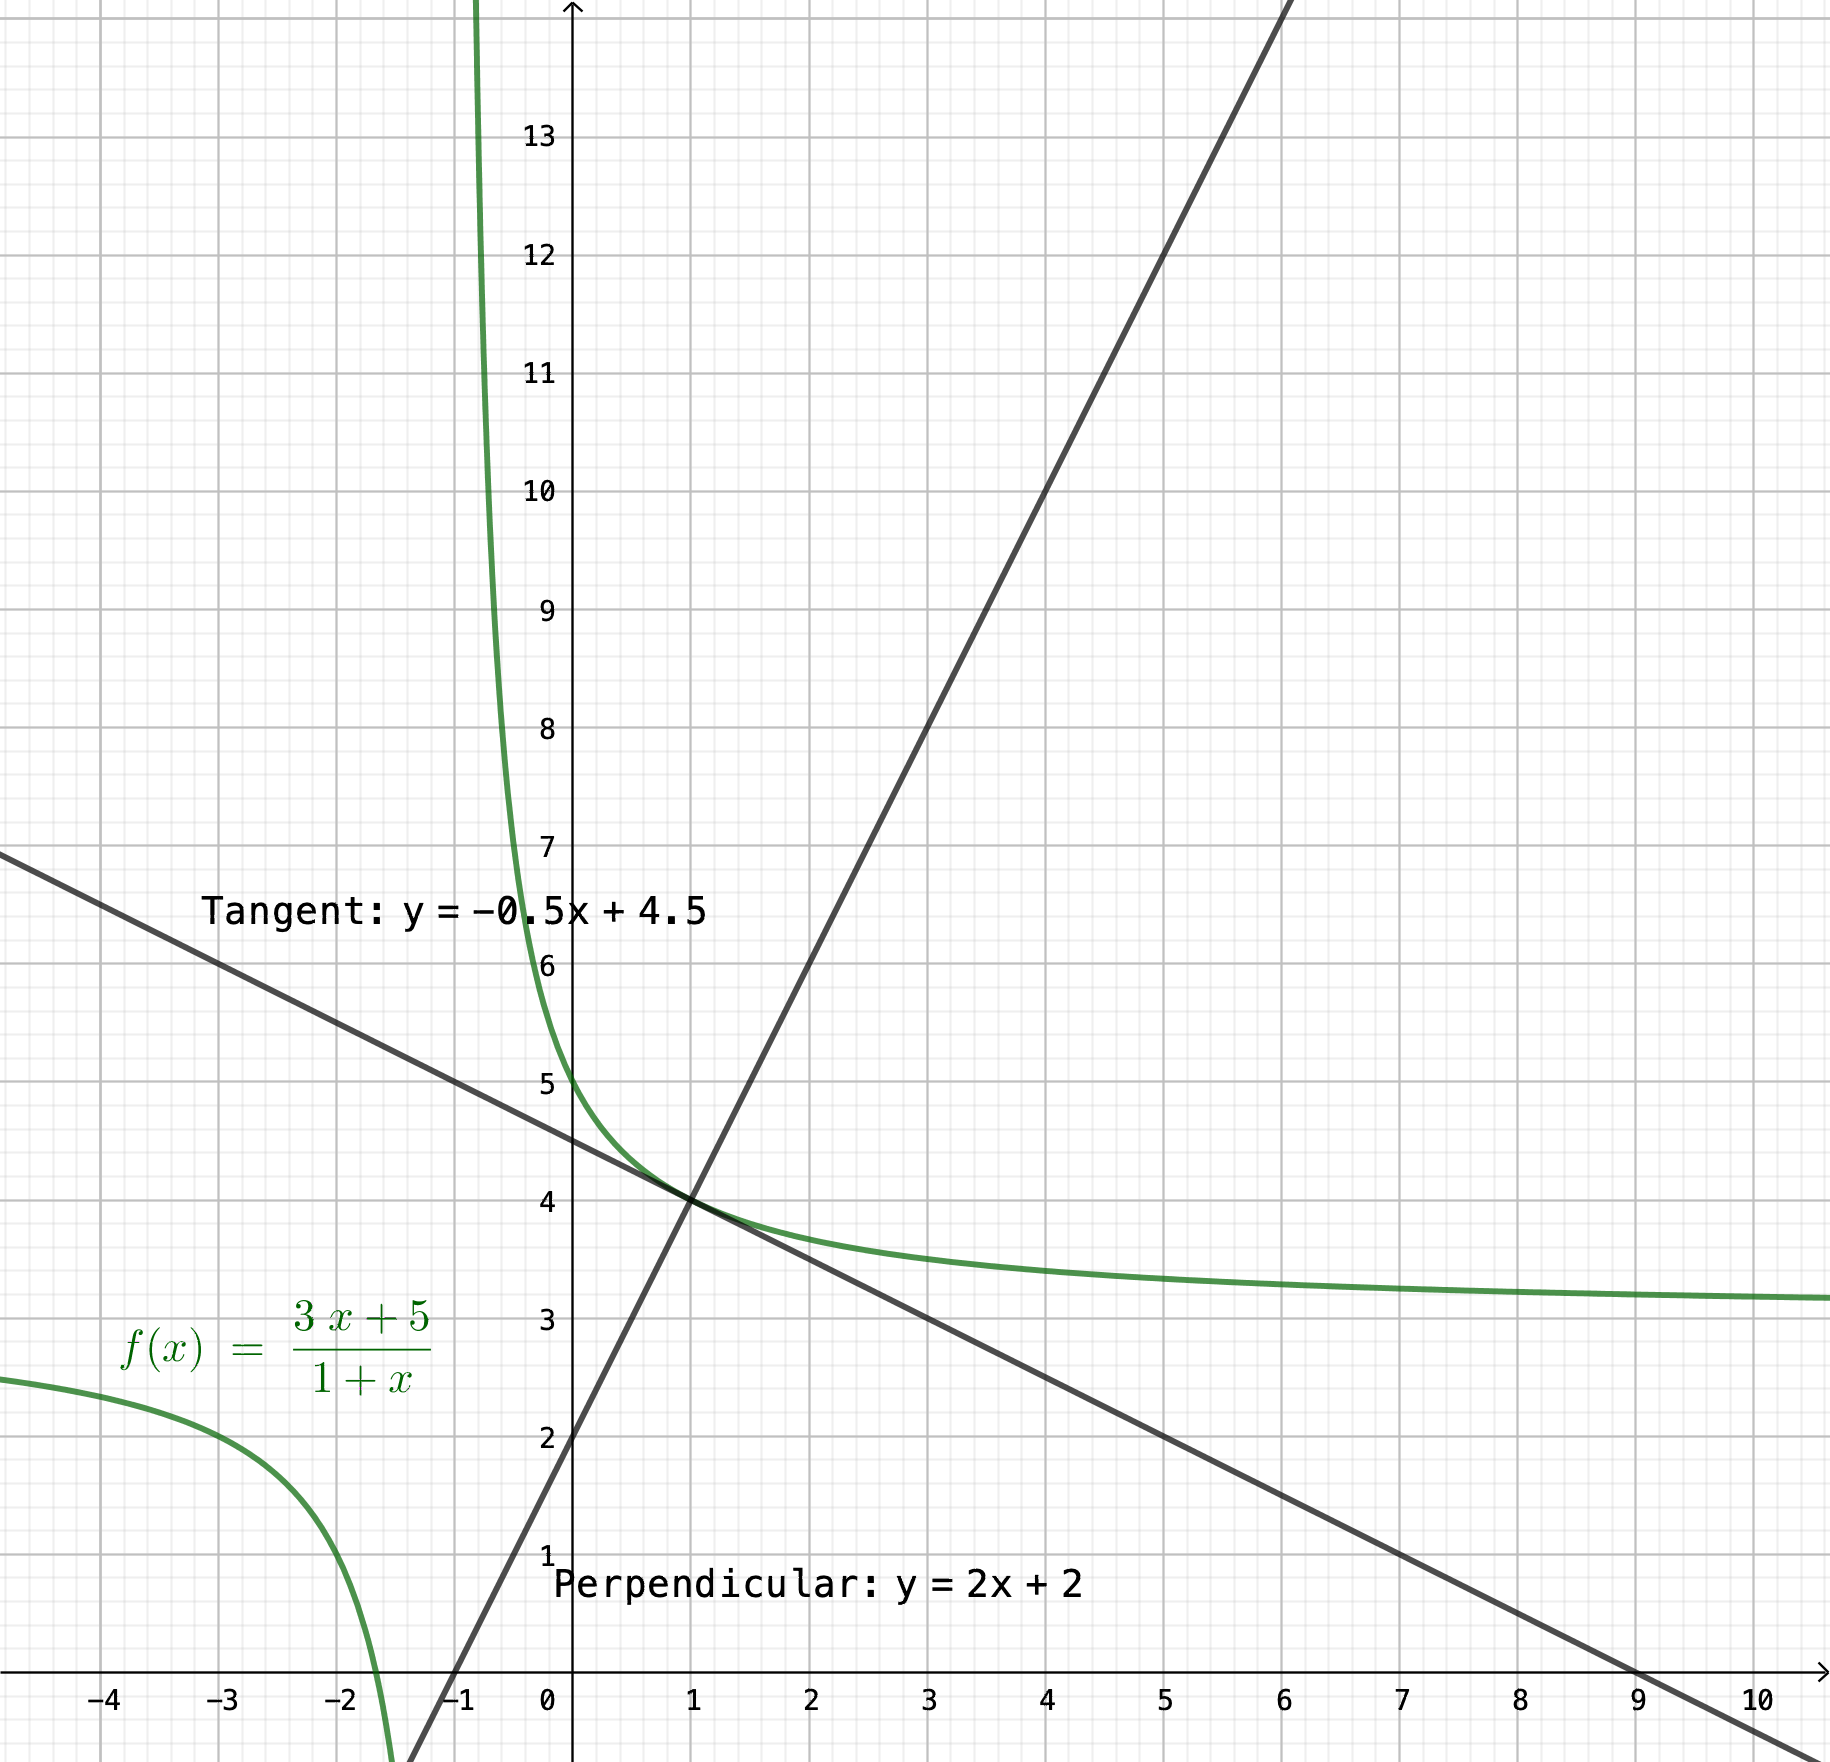
\includegraphics[width=\textwidth]{gp2-3}
\centering{Graph of $f(x)$, 3.a, and 3.b}



\end{document}
